\section{Heat and Temperature}

\subsection{Temperature and Thermal equilibrium}
When two objects are at the same temperature, they are said to be in \textbf{thermal equilibrium}. Thermal energy will flow from a hot object to a cold object until thermal equilibrium is achieved. 

\begin{definition}{(\textbf{Thermal equilibrium})}
\textit{Thermal equilibrium is the state in which there is \textbf{no net flow} of thermal energy between the objects that are involved.}
\end{definition}

\subsection{Laws of Thermodynamics}

\begin{theorem}{(\textbf{Zeroth law})}
\textit{If two systems are both in thermal equilibrium with a third system then they are in thermal equilibrium with each other.}
\end{theorem}

\begin{theorem}{(\textbf{First law})}
\textit{The increase in internal energy of a closed system is }
\begin{equation}
    \Delta U_{system} = \Delta Q - \Delta W
\end{equation}
\textit{where $\Delta U_{system}$ denotes the change in internal energy, $\Delta Q$ denotes the energy entering the system as heat and $\Delta W$ denotes the energy leaving the system as work.}
\end{theorem}
It follows from the first law of thermodynamics that in a thermodynamic cycle of a closed system $\Delta U_{system(\textit{full cycle})}$ is zero
\begin{equation}
    \Delta U_{system(\textit{full cycle})} = 0,
\end{equation}
hence 
\begin{equation}
    Q = Q_{in} - Q_{out} + W_{in} - W_{out} = W.
\end{equation}

\subsection{Temperature Scales}

In order to measure temperature, a scale is required, that includes two fixed points.\\

\noindent \textit{Celsius scale}. The Celsius scale, on the most common temperature scale, uses the freezing point and boiling point of water at atmospheric pressure $(101 \textrm{ kPa})$ are used as two fixed points, $0^{\degree C}$ and $100^{\degree C}$ respectively, with 100 increments between the points. However the Celsius scale can go below $0^{\degree C}$, yet temperature is a scalar quantity, therefore another scale is required.

\begin{notation}
\textit{Temperature in Celsius will be denoted $\theta$.}
\end{notation}

\noindent \textit{The Thermodynamic (Kelvin) scale}. The kelvin scale uses \textit{absolute zero} and the \textit{triple point of water} ($\sim  0.16^{\degree C}$) for two fixed points, $0 \textrm{ K}$ and $273.1 \textrm{ K}$ respectively.

\begin{definition}{(\textbf{Absolute Zero})}
\textit{Absolute zero is the lowest possible temperature, where the internal energy of a substance is at a minimum, therefore $E_k$ of the molecules is $E_k = 0 \textrm{ J}$.}
\end{definition}
\begin{notation}
\textit{Temperature in Kelvin will be denoted $T$.}
\end{notation}
\noindent It follows from the definition of Kelvin and Celsius that
\begin{equation}
    T \approx \theta + 273.
\end{equation}

\begin{experiment}
Using the \textbf{Pressure Law}, $P \propto T$ with a fixed mass of an ideal gas at a constant volume, estimated $0 \textrm{ K}$ in Celsius. 
\end{experiment}

\subsection{The Kinetic Model}
\label{subsection:kinetic-model}

The kinetic model describes the different phases (states) of all substances

\begin{table}[h!]
    \resizebox{17cm}{!}{
        \begin{tabular}{l|l|l|l}
            Phase & Solid & Liquid & Gas  \\
            \hline
            Density ($\rho \textrm{ kg}\mathrm{m^{-3}}$) & $900 \leq \rho \leq 3000$ & $900 \leq \rho \leq 2500$ & $0.1 \leq \rho \leq 1.5$ \\
            Atomic Spacing (m) & $\sim 10^{-10}$ & $\sim 10^{-10}$ & $\sim 10^{-9}$ \\
            Ordering & fixed, structured arrangement & less regular arrangement & random, no arrangement \\
            Motion & vibrating around a fixed point & free to flow / slide past each other & random motion \\
            Strength of electrostatic forces & strong & strong, but not as strong as solids & negligible
        \end{tabular}
    }
\end{table}
\FloatBarrier

\subsection{Internal Energy}

The internal energy of a system changes as a result of heat / energy transfer or work done by or on the system.

\begin{definition}{(\textbf{Internal Energy})}
\textit{The internal energy, $U$, is the sum of all the kinetic energies of the molecules, $E_k$, plus the potential energies, $E_p$, in the chemical bonds holding the atoms and molecules together.}
\begin{equation}
    U = E_k + E_p
\end{equation}
\end{definition}

Increasing the internal energy of a body can be described using the following graph
\begin{figure}[h!]
    \centering
    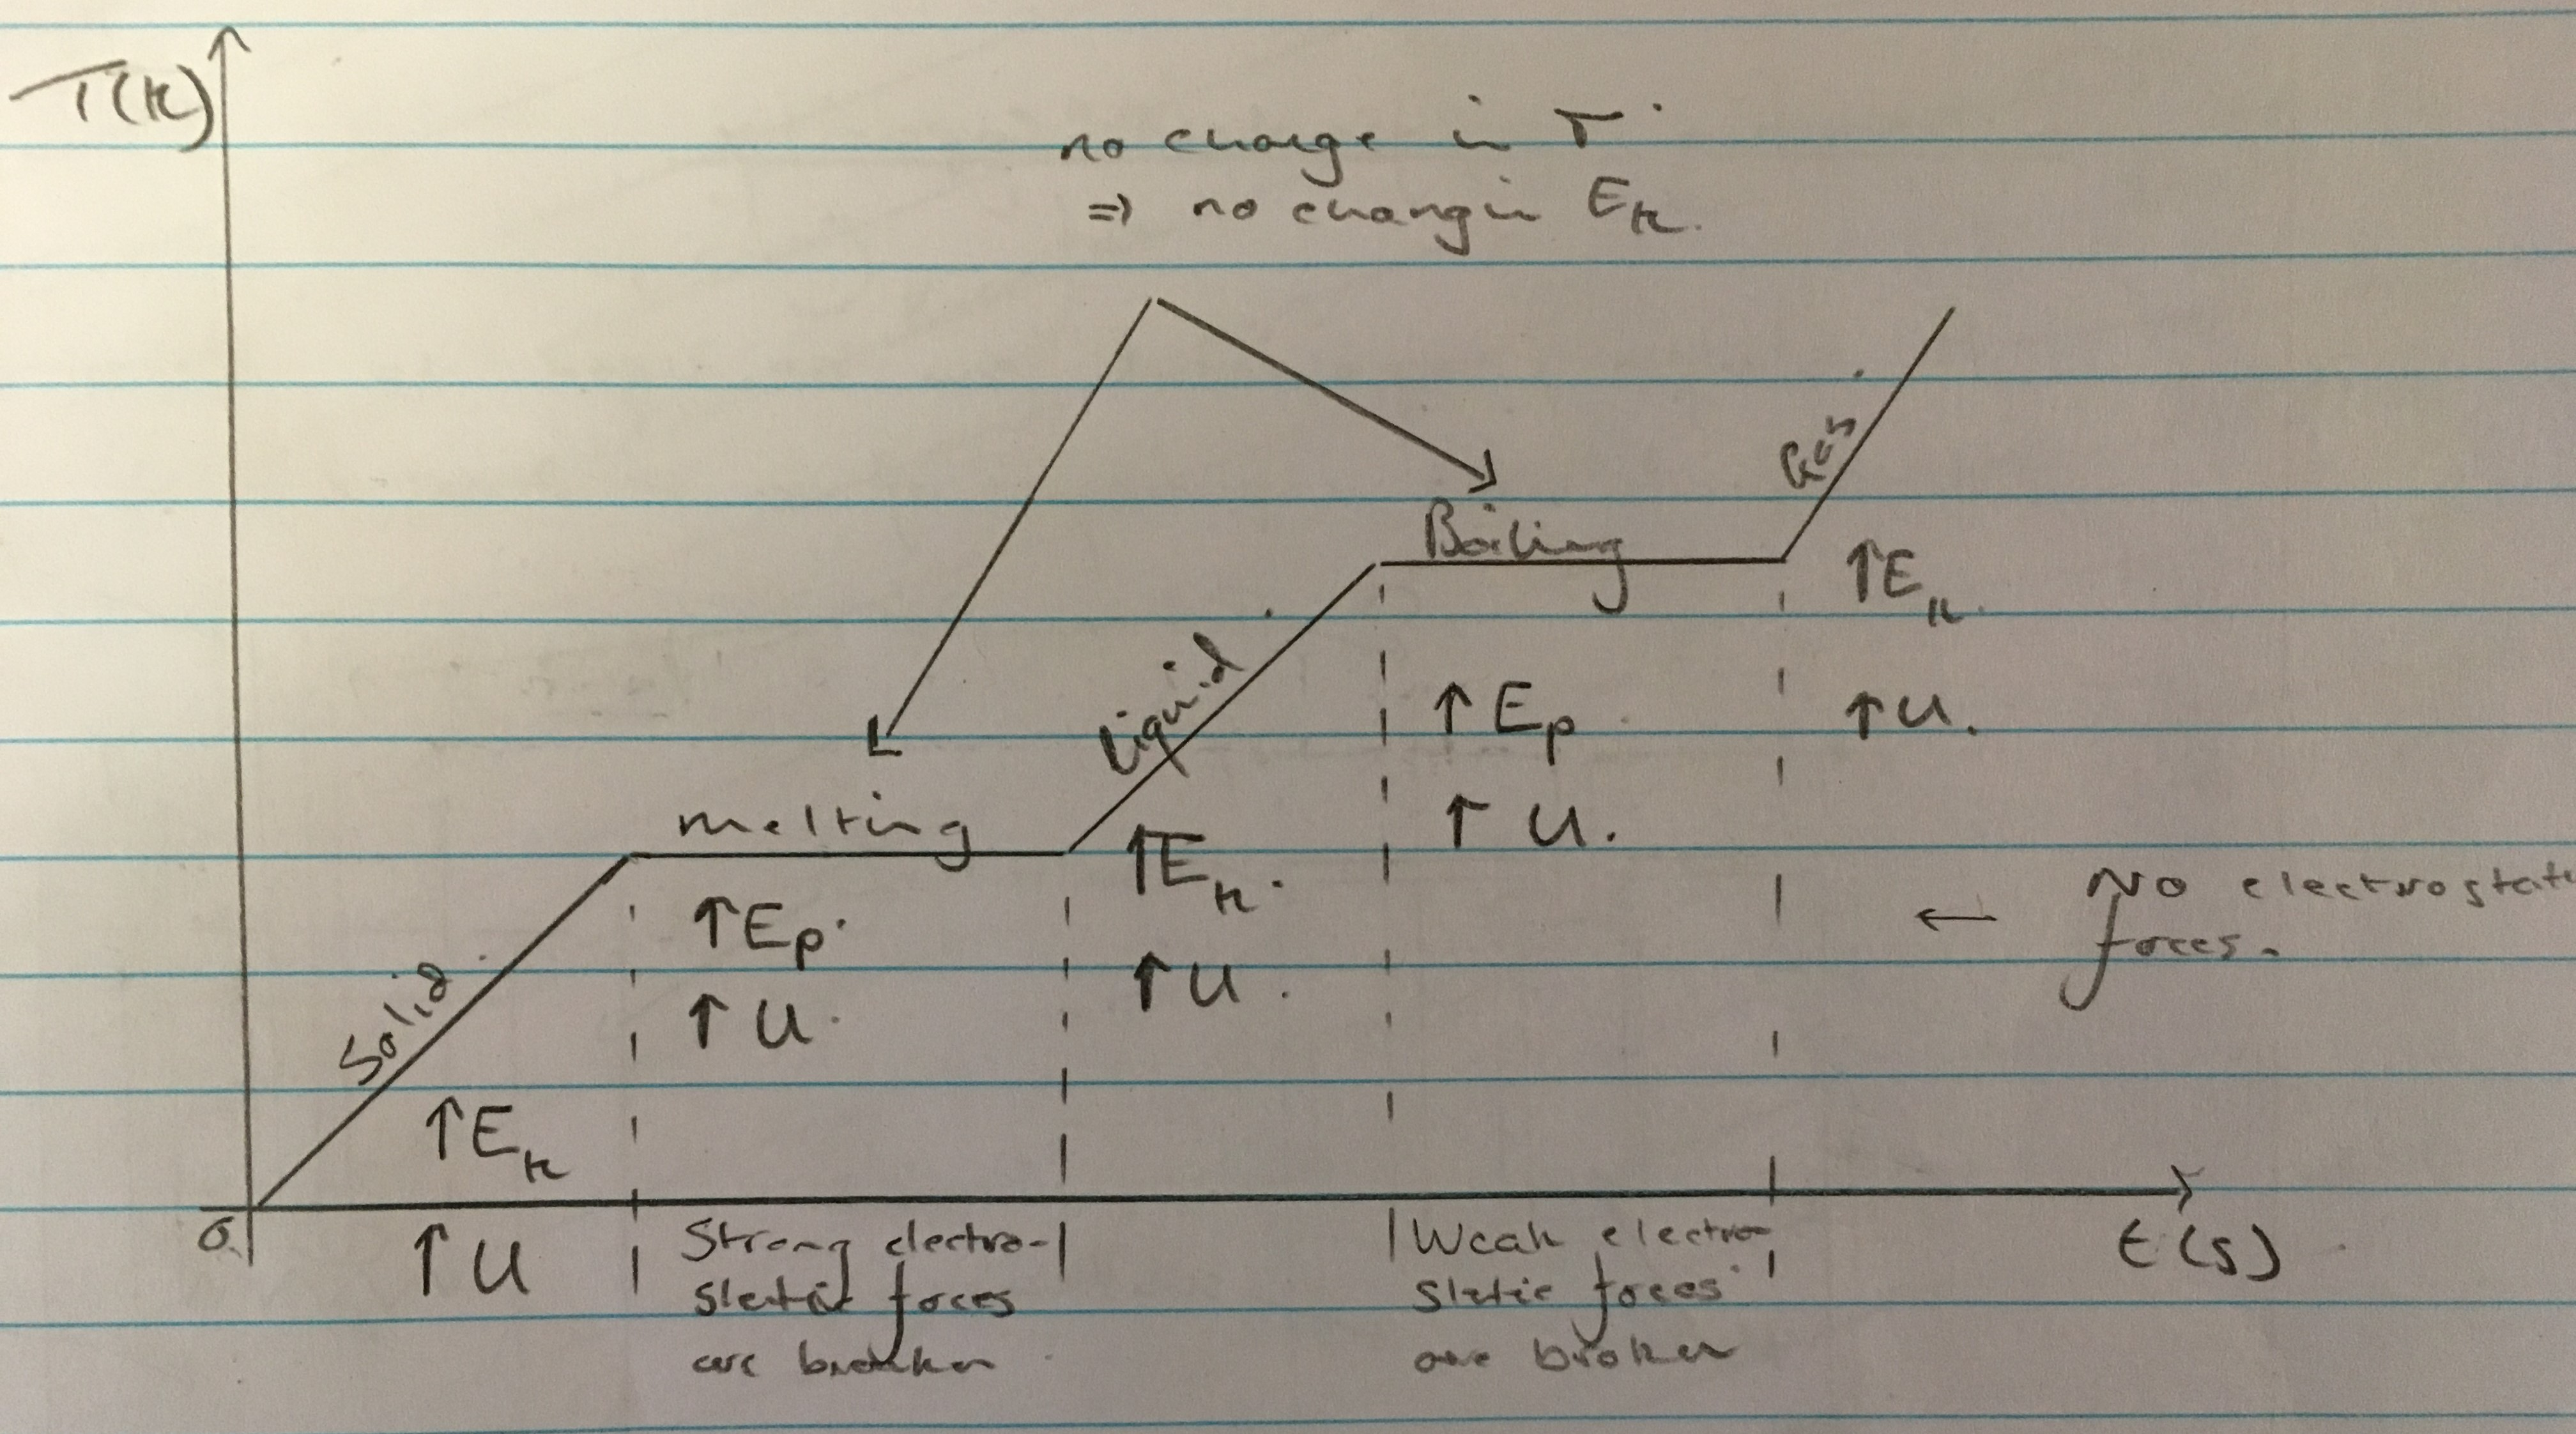
\includegraphics[scale=0.09]{notes/images/Internal-Energy-Graph-Rotated.JPG}
    \caption{Graph showing temperature against time}
\end{figure}
\FloatBarrier


\subsection{Specific Heat Capacity}
\begin{definition}{(\textbf{Specific Heat Capacity})}
\textit{The internal energy required to raise the temperature of a unit mass of a substance by a unit temperature change without change of state.}
\end{definition}

For an object of mass, $m$, with a change in temperature from $T_1$ to $T_2$ of specific heat capacity, $c$, and thermal energy change $\Delta Q$, the following applies,
\begin{equation}
    \label{eq:thermal-energy-change}
    \Delta Q = mc(T_2 - T_2)
\end{equation}
\textbf{NB:} Note that $T_1$ and $T_2$ may be in Kelvin or Celsius.

\subsubsection{Determining Specific Heat Capacity}

A simple experiment can be used to determine the specific heat capacity of a solid or liquid. Let us consider the following apparatus and circuit diagram

\begin{figure}[h!]
    \centering
    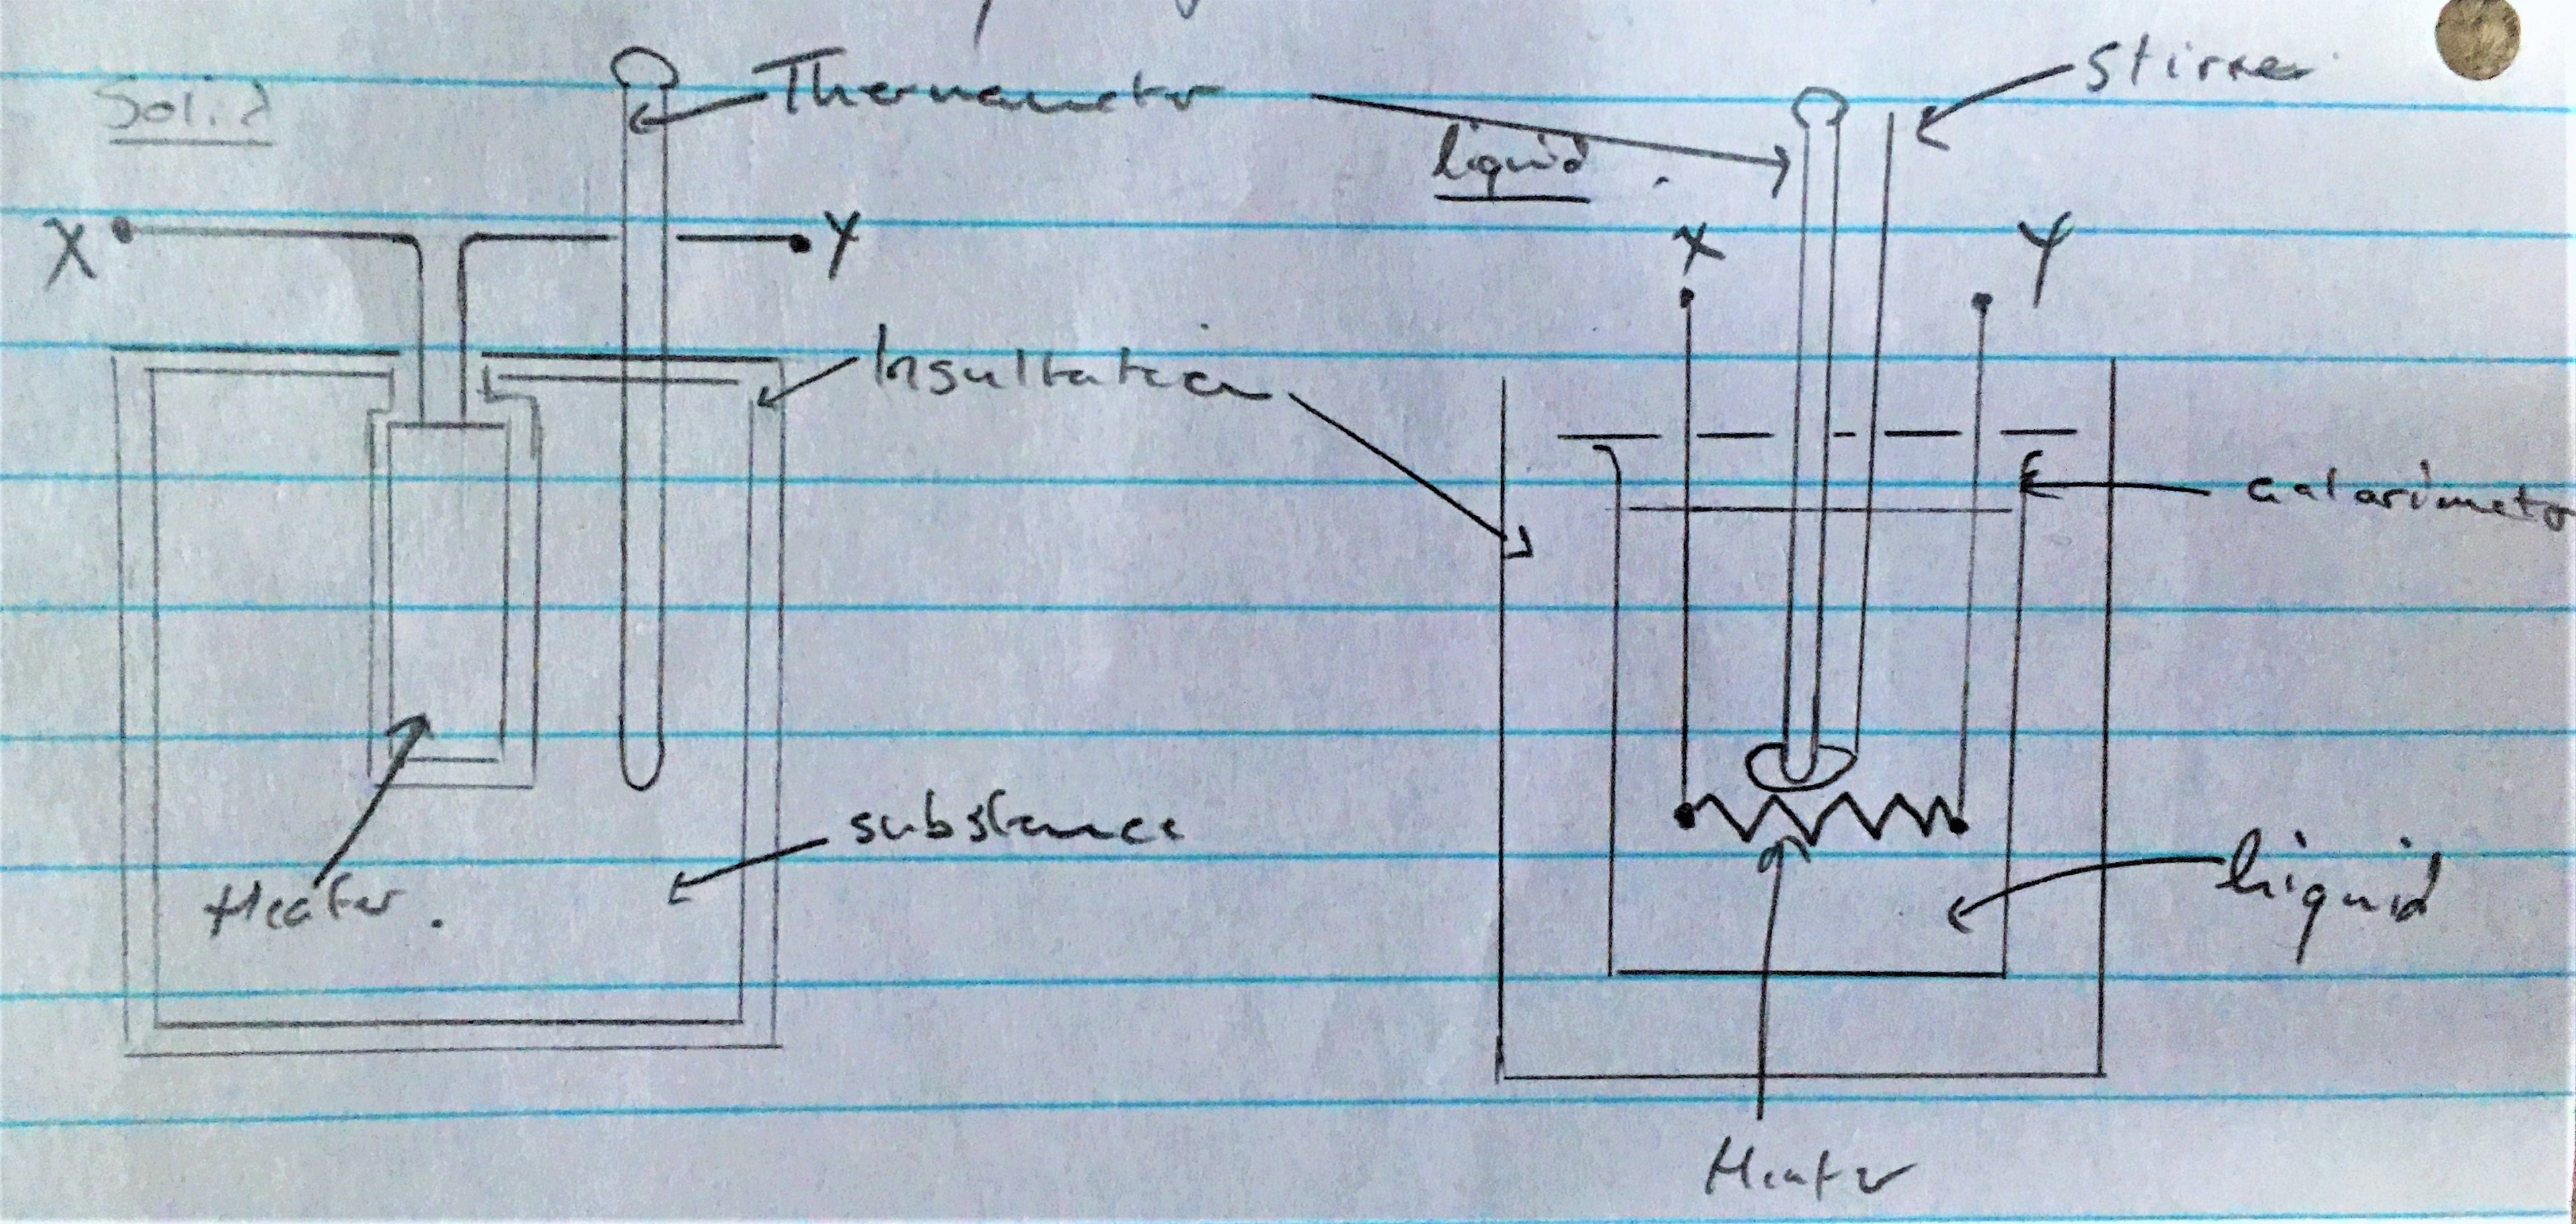
\includegraphics[scale=0.09]{notes/images/Specific-Heat-Capacity.JPG}
    \caption{Solid and liquid apparatus}
\end{figure}
\FloatBarrier

\begin{figure}[h!]
    \centering
    \begin{circuitikz}[scale=0.7]
        \draw (0,0) to [battery, ](0,4) to [ammeter, i_=$I$](4,4) to (4,0) to [short, -*](3,0) node[above] {Y};
        \draw (0,0) to [short, -*](1,0) node[above] {X};
        \draw (3.5,0) to (3.5,-2) to [voltmeter, v=$V$](0.5,-2) to (0.5,0);
    \end{circuitikz}
    \caption{Heating circuit}
\end{figure}
\FloatBarrier

From the definition of work done and electrical power, it follows that the energy inputted into the heater is given by
\begin{equation*}
    \Delta Q = VI\Delta t,
\end{equation*}
where $\Delta t$ is the amount of time required to increase the temperature from $T_1$ to $T_2$. Using equation \ref{eq:thermal-energy-change} we obtain,
\begin{equation*}
    c = \frac{VI \Delta t}{m \Delta T}.
\end{equation*}

However, this is based on the assumption of a closed system which we know not to be true in this scenario. Alternatively, we could repeat this experiment multiple times changing the final temperature $T_2$. The recorded values can then be plotted in a \textit{temperature-time} graph. Drawing a line of best fit can then be used to eliminate some of the uncertainty. For example, we might end up with a graph like this


\begin{figure}[h!]
    \centering
    \begin{tikzpicture}
    \begin{axis}[
        axis lines = left,
        xlabel = $t$,
        ylabel = $T$,
        domain=0:10,
        xmin=0, xmax=10, ymin=0, ymax=15,
        yticklabels=\empty,
        xticklabels=\empty,
        ]
        \addplot[color=red]{0.5*x + 6};
    \end{axis}
    \end{tikzpicture}
\end{figure}
\FloatBarrier

\noindent with a gradient of $k = \frac{\Delta T}{\Delta t}$. If we now consider the equation
\begin{equation*}
    \frac{\Delta Q}{\Delta t} = mc \frac{\Delta T}{\Delta t},
\end{equation*}
and use the definition of power we find that
\begin{equation*}
    P = mc \frac{\Delta T}{\Delta t}.
\end{equation*}
Rearranging this to find $c$, we get
\begin{equation*}
    c = \frac{P}{mk},
\end{equation*}
where $k$ is the gradient of the temperature-time graph and $P$ is the power supplied to the heating circuit. 

\subsection{Specific Latent Heat}

\begin{definition}{(\textbf{Specific Latent Heat})}
\textit{The specific latent heat of a substance $L$ is defined as the thermal energy $Q$ required to change the phase of a substance per unit mass while at a constant temperature; that is}
\begin{equation}
    L = \frac{Q}{m}
\end{equation}
\textit{where $m$ is the mass of the substance and $Q$ is the thermal energy required to change the phase of the substance.}
\end{definition}
\noindent There are two forms of specific latent heat: fusions and vaporization.

\begin{definition}{(\textbf{Specific Latent Heat of Fusion})}
\textit{The specific latent heat of fusion of a substance $L_f$ is defined as the thermal energy $Q$ required to melt a unit mass of the substance at it's melting point; that is}
\begin{equation}
    L_f = \frac{Q}{m}
\end{equation}
\textit{where $m$ is the mass of the substance and $Q$ is the thermal energy required to melt the substance.}
\end{definition}

\begin{definition}{(\textbf{Specific Latent Heat of Vaporization})}
\textit{The specific latent heat of vaporization of a substance $L_v$ is defined as the thermal energy $Q$ required to vaporize a unit mass of the substance at it's boiling point; that is}
\begin{equation}
    L_v = \frac{Q}{m}
\end{equation}
\textit{where $m$ is the mass of the substance and $Q$ is the thermal energy required to vaporize the substance.}
\end{definition}

\subsubsection{Determining Specific Latent Heat}

A simple experiment can be used to determine the specific latent heat of fusion or vaporization of a substance. Let us consider the following apparatus and circuit diagram

\begin{figure}[h!]
    \centering
    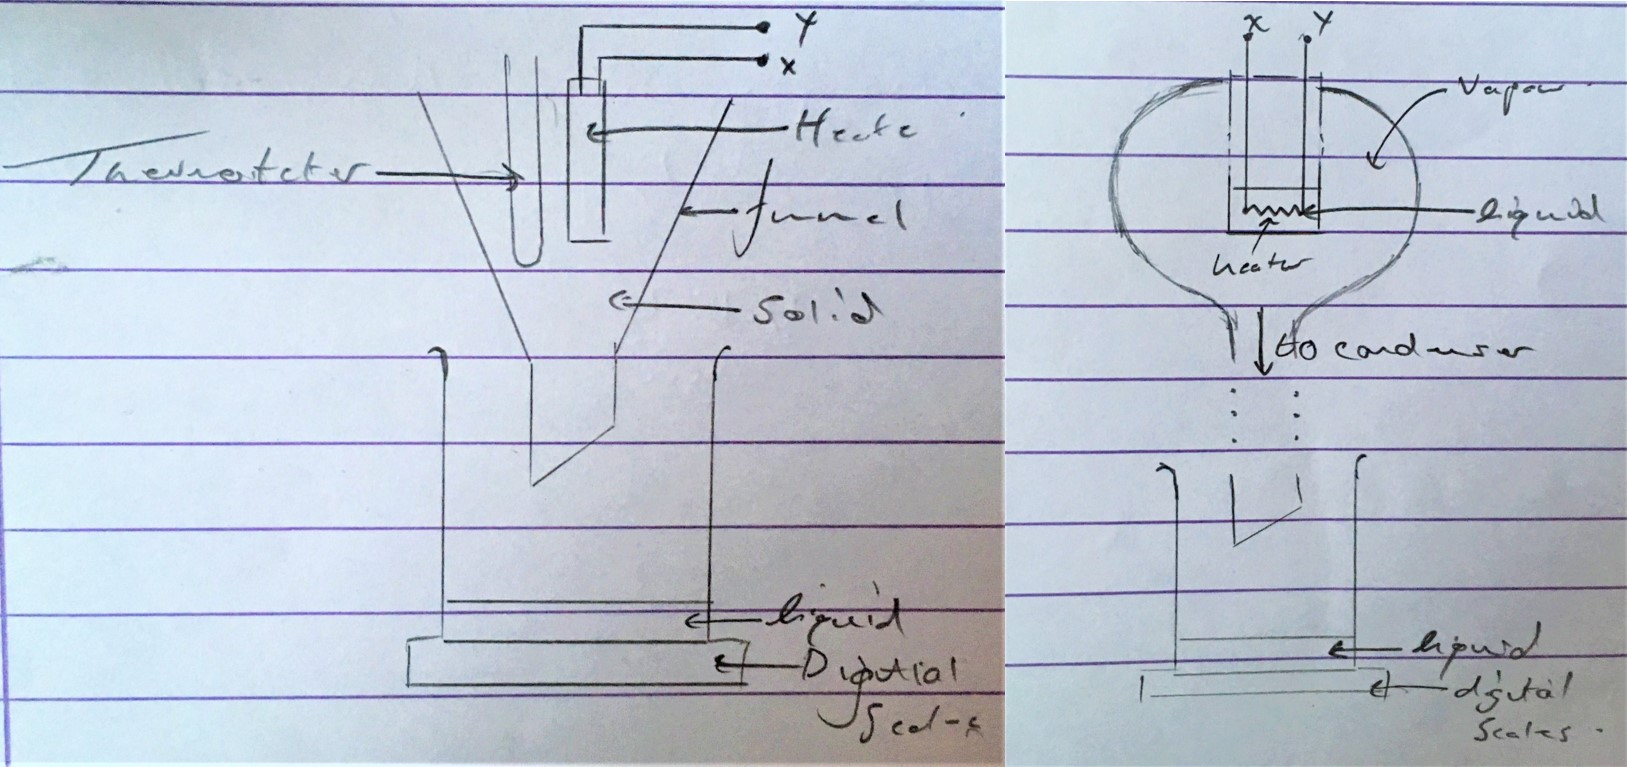
\includegraphics[scale=0.55]{notes/images/Specific-Latent-Heat.JPG}
    \caption{Solid and liquid apparatus}
\end{figure}
\FloatBarrier

\begin{figure}[h!]
    \centering
    \begin{circuitikz}[scale=0.7]
        \draw (0,0) to [battery, ](0,4) to [ammeter, i_=$I$](4,4) to (4,0) to [short, -*](3,0) node[above] {Y};
        \draw (0,0) to [short, -*](1,0) node[above] {X};
        \draw (3.5,0) to (3.5,-2) to [voltmeter, v=$V$](0.5,-2) to (0.5,0);
    \end{circuitikz}
    \caption{Heating circuit}
\end{figure}
\FloatBarrier

From the definition of work done and electrical power, it follows that the energy inputted into the heater is given by
\begin{equation*}
    Q = VI\Delta t,
\end{equation*}
where $\Delta t$ is the amount of time required to produce a change in mass $\Delta m$ in the beaker. Applying the definition of specific latent heat, we find that 
\begin{equation*}
    L = \frac{VI \Delta T}{ \Delta m}
\end{equation*}

We note that in order to obtain an accurate result the thermometer is used to ensure the solid / liquid remains at their melting / boiling points. Otherwise we would need to consider the thermal energy used to increase the temperature.

\section{Ideal Gases}

\subsection{Pressure and Kinetic Theory}

Recall from section \ref{subsection:pressure} that the definition of pressure is:

\begin{definition}{(\textbf{Pressure})}
\textit{The pressure, p, of a gas is defined as the ratio between the magnitude of the normal force $\| \vec{F}_n \|$ and the area of the surface on contact $A$, that is}
\begin{equation}
    p = \frac{\| \vec{F}_n \|}{A},
\end{equation}
\textit{measured in \textbf{pascals} ($Pa$).}
\end{definition}

The \textbf{kinetic theory of gases} is a model used to describe the behaviour of the atoms / molecules in an \textbf{ideal gas}. Real gases have complex behaviour, so in order to keep the model simple a number of assumptions are made, which are as follows:
\begin{itemize}
    \item A gas consists of a large number of particles (refers to gaseous particles only (atoms or molecules)) in random motion.
    \item The internal energy of a gas is entirely kinetic.
    \item Collisions between particles and the walls of the container are perfectly elastic.
    \item The time during collisions is negligible compared to the time between collisions.
    \item Electrostatic forces and gravitational forces are negligible between particles, except during collisions.
    \item The total volume of the atoms/molecules is negligible compared to the volume of gas.
    \item Newton's laws of motion apply to particles. So for example, according to Newton's second law of motion $\vec{F} = \frac{\mathop{\mathrm{d}\vec{p}}}{\mathop{\mathrm{d}t}}$, so the exerted on a particle $\vec{F}_{\textit{on particle}}$ from a collision is given by
    \begin{equation}
        \vec{F}_{\textit{on particle}} = \frac{-m\vec{v} - m \vec{v}}{\Delta t} = - \frac{2m\vec{v}}{\Delta t},
    \end{equation}
    and by Newton's third law of motion, the force exerted by the particle $\vec{F}_{\textit{by particle}}$ during a collision is 
    \begin{equation}
        \vec{F}_{\textit{by particle}} = \frac{2m\vec{v}}{\Delta t},
    \end{equation}
    where $\Delta t$ taken for the change in momentum to occur.
\end{itemize}


\subsection{Gas Laws}

The so-called \textbf{gas laws} state the relationships between pressure, volume and temperature of an ideal gas. The early gas laws are considered to be special cases of the \textit{ideal gas equation}, with one or more variables held constant.

\begin{theorem}{(\textbf{Boyle's Law})}
\textit{The pressure $p$ of a fixed mass of an ideal gas is inversely proportional to it's volume $V$ provided the temperature remains constant.}
\begin{equation}
    p \propto \frac{1}{V} \textit{ or } p_1 V_1 = p_2 V_2.
\end{equation}
\textit{The graph for this inverse relationship is,}
\begin{figure}[h!]
    \centering
    \begin{tikzpicture}
        \begin{axis}[
            axis lines = left,
            xlabel = $V$,
            ylabel = $p$,
            domain=0:10,
            xmin=0, xmax=10, ymin=0, ymax=15,
            yticklabels=\empty,
            xticklabels=\empty,
            samples=300,
        ]
        \addplot[color=red, restrict y to domain=0:15]   {1/(0.1 * x)} node[anchor=east,pos=0.3] {$T_1$};
        \addplot[color=black, restrict y to domain=0:15] {2/(0.1 * x)} node[anchor=east,pos=0.3] {$T_2$};
        \addplot[color=green, restrict y to domain=0:15] {4/(0.1 * x)} node[anchor=east,pos=0.3] {$T_3$};
    \end{axis}
    \end{tikzpicture}
\end{figure}
\FloatBarrier
\noindent \textit{where $T_1 > T_2 > T_3$.}
\end{theorem}

If we consider Boyle's Law, we find that the collisions frequency of the modules of a fixed mass of an ideal gas $f_{collision}$ is directly proportional to the pressure $p$, so we have
\begin{equation}
    f_{collision} \propto p \propto \frac{1}{V}.
\end{equation}

\begin{theorem}{(\textbf{Charles' Law})}
\textit{The volume $V$ of a fixed mass of an ideal gas is proportional to it's temperature $T$ provided the pressure remains constant.}
\begin{equation}
    V \propto T \textit{ or } \frac{V_1}{T_1} = \frac{V_2}{T_2}.
\end{equation}
\textit{The graph for this relationship is,}
\begin{figure}[h!]
    \centering
    \begin{tikzpicture}
        \begin{axis}[
            axis lines = left,
            xlabel = $T$,
            ylabel = $V$,
            domain=0:10,
            xmin=0, xmax=10, ymin=0, ymax=15,
            yticklabels=\empty,
            xticklabels=\empty,
            samples=300,
        ]
        \addplot[color=red, restrict y to domain=0:15]   {2 * x} node[anchor=east,above,pos=0.9] {$N_1$};
        \addplot[color=black, restrict y to domain=0:15] {0.5 * x} node[anchor=east,above,pos=0.9] {$N_2$};
    \end{axis}
    \end{tikzpicture}
\end{figure}
\FloatBarrier
\noindent \textit{where $N_2 > N_1$ and $N$ denotes the number of molecules in the fixed mass of the ideal gas.}
\end{theorem}

\begin{theorem}{(\textbf{The Pressure Law})}
\textit{The pressure $p$ of a fixed mass of an ideal gas is proportional to it's temperature $T$ provided the volume remains constant.}
\begin{equation}
    p \propto T \textit{ or } \frac{p_1}{T_1} = \frac{p_2}{T_2}.
\end{equation}
\textit{The graph for this relationship is,}
\begin{figure}[h!]
    \centering
    \begin{tikzpicture}
        \begin{axis}[
            axis lines = left,
            xlabel = $T$,
            ylabel = $p$,
            domain=0:10,
            xmin=0, xmax=10, ymin=0, ymax=15,
            yticklabels=\empty,
            xticklabels=\empty,
            samples=300,
        ]
        \addplot[color=red, restrict y to domain=0:15]   {2 * x} node[anchor=east,above,pos=0.9] {$N_1$};
        \addplot[color=black, restrict y to domain=0:15] {0.5 * x} node[anchor=east,above,pos=0.9] {$N_2$};
    \end{axis}
    \end{tikzpicture}
\end{figure}
\FloatBarrier
\noindent \textit{where $N_2 > N_1$ and $N$ denotes the number of molecules in the fixed mass of the ideal gas.}
\end{theorem}

\subsection{The Ideal Gas Law}
The \textbf{combined gas equation} is a good approximation of the behaviour of a fixed mass of an ideal gas with no constant variables, however it has several limitations; one being that it only works for a fixed mass of an ideal gas. It is a combination of the empirical Boyle's Law, Charles' Law and the Pressure Law and is written as
\begin{equation}
    \frac{p_1 V_1}{T_1} = \frac{p_2 V_2}{T_2}.
\end{equation}

However, the \textbf{ideal gas law}, also called the \textbf{equation of state} of an ideal gas, is an approximation of the behaviour of many ideal gases under many conditions (i.e. a mass changing system). The equation of state is often written as 
\begin{equation}
    pV = nRT,
\end{equation}
where $p$, $V$, $T$ are the pressure, volume and absolute temperature; $n$ is the number of moles of gas and $R$ is the \textbf{ideal gas constant}. It is the same for all \textit{ideal} gases. The equation of state is frequently written in other forms such as
\begin{equation}
    pV = N k_B T \text{ and } \frac{pV}{T} = nR = N k_B,
\end{equation}
where $k_B$ is the Boltzmann constant. We note the definition of the Boltzmann constant (named after Ludwig Boltzmann) $k_B$ is equivalent to the ideal gas constant $R$ divides by Avogadro's constant $N_A$. Mathematically, we have
\begin{equation}
    \label{eq:boltzmann-constant}
    k_B = \frac{R}{N_A} = \frac{nR}{N} \approx 1.38 \times 10^{-23},
\end{equation}
measured in \textbf{joules per kelvin} ($JK^{-1}$) and where $n$, $N$ denotes the number of moles and molecules, respectively. \\

We will now consider the empirical derivation of the equation of state of an ideal gas with parameters $p_1$, $V_1$, $N_1$ and $T_1$, where $N$ denotes the number of molecules of the ideal gas. Keep in mind, to understand this derivation, one must imagine the gas being altered by one process at a tiime. We first state Boyle's Law, then we have 
\begin{equation*}
    p_1 V_1 = p_2 V_2.    
\end{equation*}
After this process, the gas has the parameters $p_2$, $V_2$, $N_1$ and $T_1$. We now consider a change in temperature and the number of molecules in the gas, we note the relationship $NT = \text{constant}$, so we have 
\begin{equation*}
    N_1 T_1 = N_2 T_2,
\end{equation*} 
so the gas now has the parameters $p_2$, $V_2$, $N_2$ and $T_2$. The change in pressure and the number of particles is given by the following relationship 
\begin{equation*}
    \frac{p_2}{N_2} = \frac{p_3}{N_3},
\end{equation*} 
so we now have the following parameters: $p_3$, $V_2$, $N_3$ and $T_2$. Applying Charles' Law to change the volume and temperature of the gas, we have
\begin{equation*}
    \frac{V_2}{T_2} = \frac{V_3}{T_3}.
\end{equation*}
Using simple algebra on these relations yields the result;
\begin{equation*}
    \frac{p_1 V_1}{N_1 T_1} = \frac{p_2 V_2}{N_2 T_2} \text{ or } \frac{pV}{T} = N k_B.
\end{equation*}
Which is a general case of the combined gas equation we initially stated in this section. Another equivalent result (from equation \ref{eq:boltzmann-constant}) is 
\begin{equation*}
    \frac{pV}{T} = nR,
\end{equation*}
which is known as the \textbf{ideal gas law}.

\subsection{The Maxwell-Boltzmann Distribution}

In Physics, specifically statistical mechanics, the \textbf{Maxwell-Boltzmann distribution} is a probability distribution used for describing the particle speeds in idealized gases. The Mathematics behind the Maxwell-Boltzmann distribution are based on a chi distribution with three degrees of freedom (the components of the velocity vector in the Euclidean space $\mathbf{E}^3$), however since statistics is tedious and boring; we shall go no further than this for understanding why the Maxwell-Boltzmann distribution works. In this course, we shall only consider the mean speeds of particles according to this distribution. The mean speed $\overline{v}$, most probable speed $v_p$ and root-mean-square speed $\sqrt{\overline{v^2}}$ can be obtained from properties of the Maxwell-Boltzmann distribution, however, we will only consider the root-mean-square speed and it's relationship to pressure at a microscopic scale. 

In order to obtain root-mean-square speed of a gas, the velocities of the each particle $\vec{v_1}, \vec{v_2}, \ldots, \vec{v_n}$ are required. We then average the square the components of these velocities in a single dimension to find the mean-square speeds of the gas $\overline{v_{i}^2}$ in the $i^{th}$ dimension, that is
\begin{equation}
    \overline{v_{i}^2} = \frac{1}{n} \sum_{k=1}^n v_{k, i}^2.
\end{equation}
We now must consider the fact that we have a collection of particles moving with a range of speeds in random directions. Any particle may have its velocity $\vec{v}$ resolved into three perpendicular components. We may resolve the mean-square speeds in the same way, so that:
\begin{equation*}
    \overline{v^2} = \overline{v_x^2} + \overline{v_y^2} + \overline{v_z^2}.
\end{equation*}
By definition, the root-mean-square speed $\sqrt{\overline{v^2}}$, sometimes denoted $v_{rms}$, is simply the square root of the mean-square speed, so we have
\begin{equation}
    v_{rms} = \sqrt{\overline{v^2}} = \sqrt{\overline{v_x^2} + \overline{v_y^2} + \overline{v_z^2}} = \sqrt{\frac{1}{n} \sum_{k=1}^n \| \vec{v_k} \|^2}.
\end{equation}
We should also note, that since there are a large number of particles in a gas and they are all moving in random directions, it follows that \textit{on average} the mean-square speeds in the $x$, $y$ and $z$ directions are all equal, that is
\begin{equation*}
    \overline{v_x^2} = \overline{v_y^2} = \overline{v_z^2},
\end{equation*}
it follows from this that we have
\begin{equation*}
    \overline{v_x^2} = \overline{v_y^2} = \overline{v_z^2} = \frac{1}{3} \overline{v^2}.
\end{equation*}

Our interest in root-mean-square speed is motivated by considering the average velocity of a gas. If we calculated the average velocity of the particles in a gas, because velocity is a vector the average would be $0$ $ms^{-1}$. So in order to describe the typical motion of particles inside the gas, we use a different measure, the root-mean-square speed, it also happens to appear in the equation
\begin{equation}
    pV = \frac{1}{3}Nm\overline{v^2},
\end{equation}
where $p$ is the pressure exerted by the gas, $V$ is the vole of the gas, $N$ is the number of particles in the gas, $m$ is the mass of each particle and $\overline{v^2}$ is the mean-square speed of the particles. This equation which refers to pressure at the microscopic level will be discussed below. 

\subsubsection{Pressure at the microscopic level}

Imagine a single particle colliding with a container wall at a normal. The container is a cube with sides $\ell$. The gas particle has a mass $m$ and velocity $v_{x, 1}$. 

\begin{figure}[h!]
    \centering
    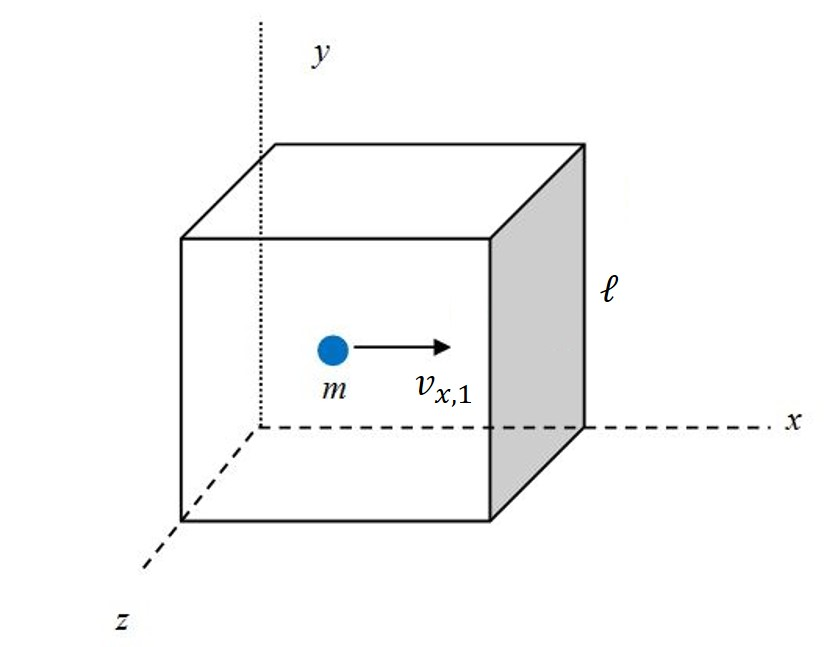
\includegraphics[scale=0.75]{notes/images/Particle-In-Box.JPG}
    \caption{Particle in a container}
\end{figure}
\FloatBarrier

The elastic collision results in a change in momentum of a magnitude of $2 m v_{x, 1}$. This process causes a force to be exerted on the wall by Newton's second law of motion and Newton's third law tells us that the wall exerts an equal and opposite forces on the particle. The particle bounces backwards and forwards between the two walls, exerting a force on each. Since velocity is defined as the first time derivative of displacement, the time $\Delta t$ between two successive collisions with a given contain wall is
\begin{equation*}
    \Delta t = \frac{2 \ell}{v_{x, 1}}.
\end{equation*}
This implies that over a time interval of $\Delta t$, the particle makes a single collision with a given container wall, in which a change of momentum of magnitude $2mv_{x, 1}$ occurs. By Newton's second law of motion, the magnitude of the force exerted by this particle on a given container wall is 
\begin{equation*}
    \| \vec{F}_{x, 1} \| = \frac{m v_{x,1}^2}{\ell}.
\end{equation*}
From the definition of pressure, we can express the pressure $p_1$ exerted by the particle on a given container wall as
\begin{equation*}
    p_1 = \frac{m v_{x,1}^2}{\ell^3}. 
\end{equation*}
Now consider there are $N$ particles, all with velocities along the $x$ dimension. All of these particles moves in a similar motion to the first particle we've been considering. Their velocities will be $v_{x, 1}, v_{x, 2}, \ldots, v_{x, N}$ respectively. Each particle exerts a pressure on the container wall we've been considering in the same way as the first particle. The total pressure $p$ exerted by all $N$ particles on the wall will be the sum of the individual pressure by each particle: 
\begin{align*}
    p &= \sum_{k=1}^N p_k \\
    &= \frac{m}{\ell^3} \sum_{k=1}^N v_{x, k}^2 \\
    &= \frac{m}{\ell^3} N \overline{v_x^2}.
\end{align*}
Applying the following relationship (after considering the fact that we have a collection of particles moving with a range of speeds in random directions):
\begin{equation*}
    \overline{v_x^2} = \overline{v_y^2} = \overline{v_z^2} = \frac{1}{3} \overline{v^2},
\end{equation*}
we find that the total pressure exerted on a single container wall (and indeed on any of the other five walls) is given by
\begin{equation*}
    p = \frac{Nm\overline{v^2}}{3 \ell^3},
\end{equation*}
we also note that $\ell^3$ is equal to the volume of the container $V$, so we have
\begin{equation}
    pV = \frac{1}{3} Nm\overline{v^2}.
\end{equation}

\subsection{Mean Kinetic Energy}

We now have two equations that describe he behaviour of a gas, one based on parameters of a gas and one based on a mechanical model of the particles in the gas. So we have
\begin{align*}
    pV &= nRT = N k_B T \\
    pV &= \frac{1}{3} Nm\overline{v^2}.
\end{align*}
Equating these, we find that
\begin{equation*}
    \frac{1}{2} m \overline{v^2} = \frac{3}{2} k_B T
\end{equation*}
The mean kinetic energy of the gas particles $\overline{E_k}$ is $\frac{1}{2} m \overline{v^2}$, so we have
\begin{equation}
    \overline{E_k} = \frac{3}{2} k_B T.
\end{equation}
Since all other values apart from $T$ remain constant in this equation, it follows that
\begin{equation}
    \overline{E_k} \propto T.
\end{equation}
Note that this only applies when using the absolute temperature (i.e. when the temperature is measured in kelvin). Also based on the assumption that the internal energy $U$ of a gas is entirely kinetic, we find
\begin{equation}
    U = \frac{3}{2} k_B T,
\end{equation}
so the internal energy of a gas is also proportional to it's temperature. 

\section{Material and Properties}